\chapter{Entorno y herramientas}
\label{cap:entorno}
En este capítulo se presentaran y describirán las herramientas hardware y software que se han usado para el desarrollo del proyecto. En primer lugar se presentará el robot sobre el que hemos trabajado, el robot kobuki. En segundo lugar se presentará el \textit{framework} sobre el que hemos construido el algoritmo, ROS , y por ultimo se describirán las herramientas de dicho framework que han resultado esenciales para la realización del proyecto.


\section{Robot Kobuki}
\label{cap:robot}
El robot kobuki o Turtlebot es un robot \textit{lowcost} que cuenta con un software de código abierto. Su estructura principal es una base móvil de forma circular y una serie de baldas y barras metálicas para adaptar su configuración física a nuestras necesidades. Cuenta con una integración total con ROS, el framework que se usará para el proyecto, y además es el robot usado por la mayoría de alumnos de la universidad para cursar la asignatura de robótica.
\begin{figure} [H]
  \begin{center}
    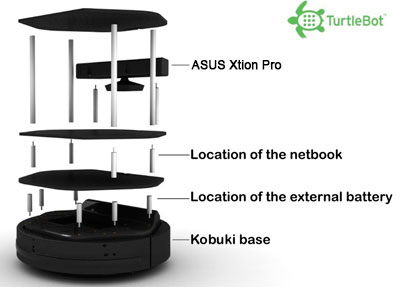
\includegraphics[width=7.5cm]{img/cap3/kobuki}
  \end{center}
  \caption{Robot kobuki.}
  \label{fig:kobuki}
\end{figure}


\section{ROS}
\label{cap:ros}


\section{Software en ROS para el mapeado, localización y navegación}
\label{cap:softwarederos}
En esta sección se describirá el funcionamiento de los diferentes paquetes que ROS nos proporciona y que resultan esenciales para la creación de mapas, la localización y la navegación por distintos entornos.

\subsection{Costmap\_2D}
\label{sec:costmap2d}
Un \textit{costmap} es una estructura de datos ofrecida por ROS y compuesta por un grid de ocupación y los metadatos de este grid. Cada celda del grid toma valores entre 0 y 255, donde 0 corresponde a una celda vacía, los valores entre 1 y 254 representan la probabilidad de que una celda está ocupada y el valor 255 se reserva para el total desconocimiento sobre el estado de una celda. Cada valor se asocia con un nivel de gris, como se puede ver en la imagen.
\begin{figure} [H]
  \begin{center}
    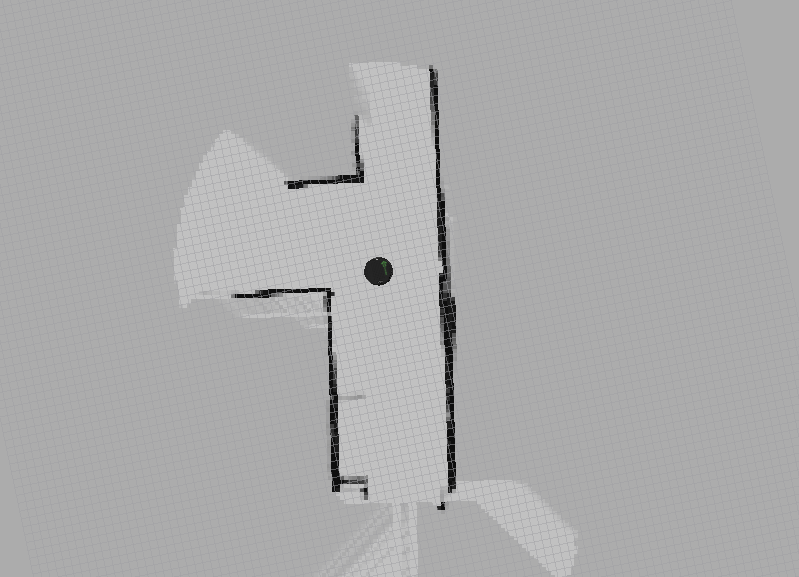
\includegraphics[width=7.5cm]{img/cap3/costmap-ejemplo}
  \end{center}
  \caption{Ejemplo visual de un costmap.}
  \label{fig:costmap-ejemplo}
\end{figure}\

Para poder representar la ocupación de un objeto en un \textit{costmap} es necesario hacer uso de las transformadas entre frames que nos ofrece ROS.

\subsubsection{tf}
\label{subsubsec:tf}
Cualquier robot está compuesto por multitud de piezas móviles, como puede ser la propia base del robot o la pinza de un brazo robótico. Cada una de estas piezas se pueden representar con un \textit{frame}. Ademas existen también otros \textit{frames} que pueden interesarnos, como puede ser el \textit{frame} de world o el \textit{frame} de map.
\begin{figure} [hbtp]
  \begin{center}
    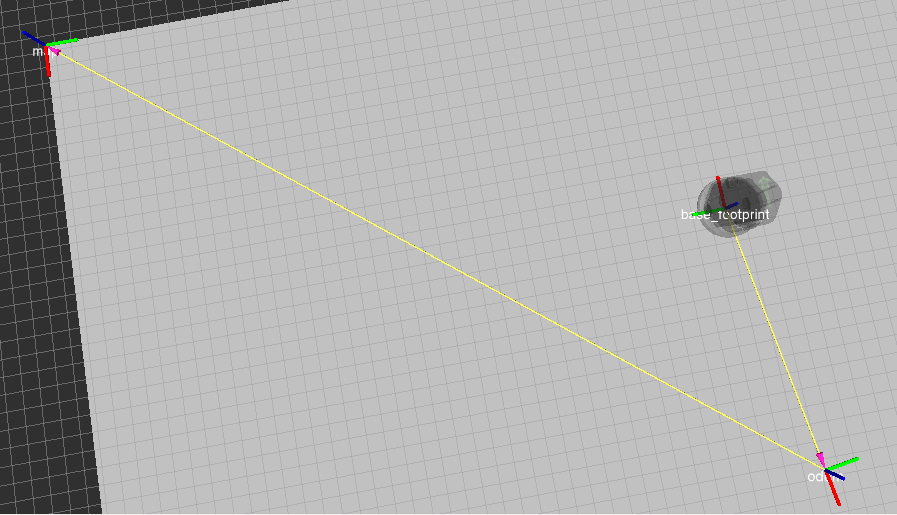
\includegraphics[width=12cm]{img/cap3/frames}
  \end{center}
  \caption{A la izquierda el frame map y a la derecha los frames de odom y base\_footprint}
  \label{fig:frames}
\end{figure}

Usamos las \textit{tf} para poder representar información relativa a uno de estos frames. Esto puede sernos de utilidad, por ejemplo, si queremos conocer la posición de un objeto que hemos cogido con nuestra pinza respecto a la base de nuestro robot, o cual es la posición relativa de un objeto que estamos percibiendo con el láser respecto a nosotros o respecto al mapa.

Cuando trabajamos con mapas es importante que todo lo que se representa en él sea respecto al frame \textit{map}. De este modo nuestro mapa puede ser usado por otros nodos, como el nodo de navegación, o por otro robot situado en el escenario representado en el mapa.


\subsection{AMCL}
\label{sec:amcl}
\textit{AMCL}\footnote{http://wiki.ros.org/amcl} es un paquete de localización que implementa un algoritmo de Monte Carlo, el cual usa un filtro de partículas para localizar al robot sobre un mapa que previamente le proporcionamos.
\subsubsection{Filtro de partículas}
El algoritmo del filtro de partículas se divide en 4 etapas: Inicialización, actualización, estimación y predicción. 
En la etapa de inicialización se ``lanzan'' una serie de partículas cercanas a la posición inicial del robot. Estas partículas ademas de una posición en el espacio también tendrán una dirección. Podemos ver un ejemplo gráfico en la imagen \ref{fig:initamcl}

\begin{figure}[hbtp]
  \begin{center}
    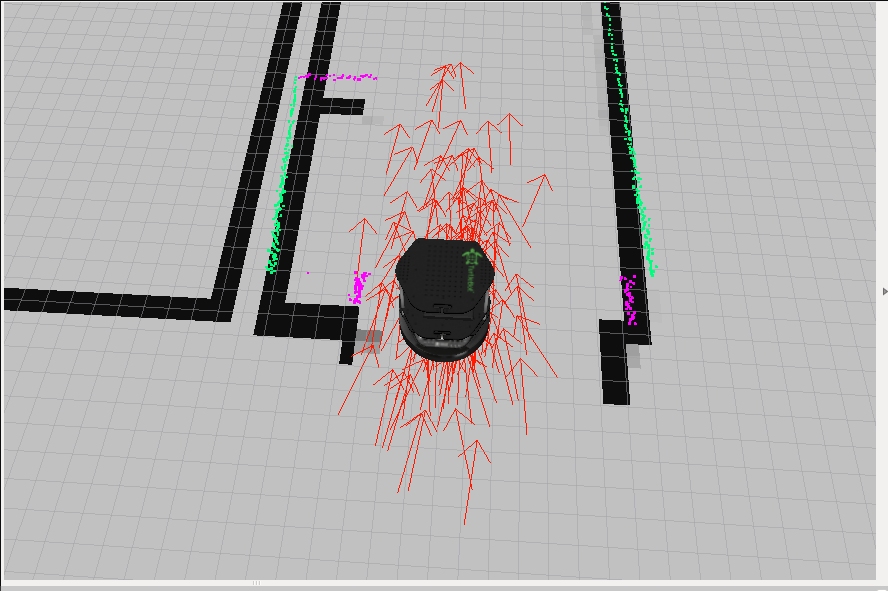
\includegraphics[width=10cm,height=7cm]{img/cap3/initamcl}
  \end{center}
  \caption{Inicialización del filtro de partículas}
  \label{fig:initamcl}
\end{figure}
Vemos como se han generado muchas partículas alrededor del robot y que cada una tiene una dirección más o menos acertada con la dirección del robot.

En este punto del algoritmo se compara la percepción del láser del robot en el punto en el que se encuentra con la percepción que tendría si tuviera la posición y la dirección de cada una de las partículas que generamos. Cuanto más acertada sea la suposición anterior, más valor se le da a esa partícula. Así nos encontraremos que las partículas que están más cercanas a la posición del robot cobran más valor y las que están más lejos y con una dirección totalmente errónea tienen menos valor. Esta fase es la llamada de Actualización. 

En la siguiente fase, llamada de Estimación, nos quedamos con las partículas que más valor tenían para volver a lanzarlas en la siguiente fase del algoritmo.

En la ultima fase, fase de Predicción, lanzamos las partículas de nuevo con el valor que tenían y su posición, añadiéndole un pequeño ruido.
En este punto del algoritmo también se corrige la posición del robot a la posición de la partícula con más valor.
Una vez completado el algoritmo se vuelve a la fase de Actualización y se repite hasta que el robot esté perfectamente localizado en el 
mapa.

\begin{figure}[hbtp]
  \begin{center}
    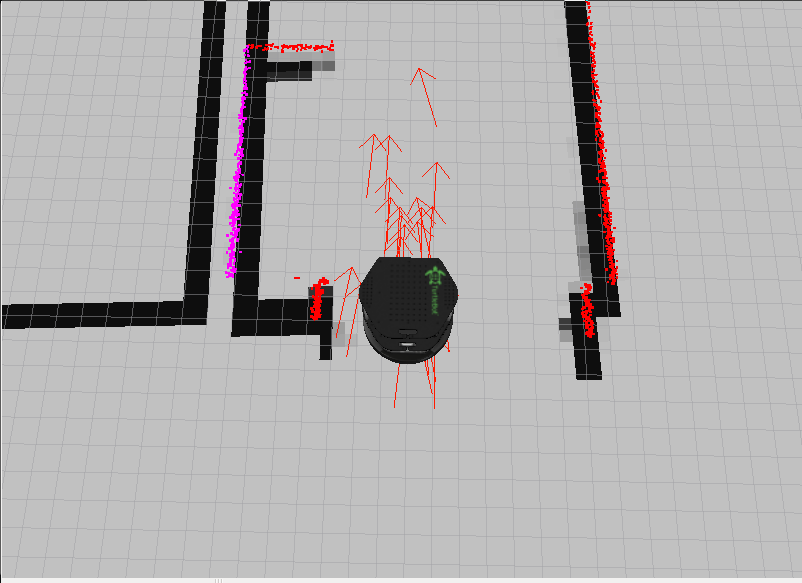
\includegraphics[width=10cm,height=7cm]{img/cap3/actamcl}
  \end{center}
  \caption{El robot se vá acercando a la posición ideal}
  \label{fig:actamcl}
\end{figure}

Observamos como la linea color de la parte derecha de la imagen \ref{fig:actamcl}, correspondiente a las muestras tomadas con el láser, está más cerca de la linea del mapa que en la imagen \ref{fig:initamcl} que se aprecia que no está alineada. Esto es fruto de la corrección que se va haciendo de la posición. También observamos que hay menos partículas, esto es fruto de la convergencia hacia la posición correcta.

\begin{figure}[hbtp]
  \begin{center}
    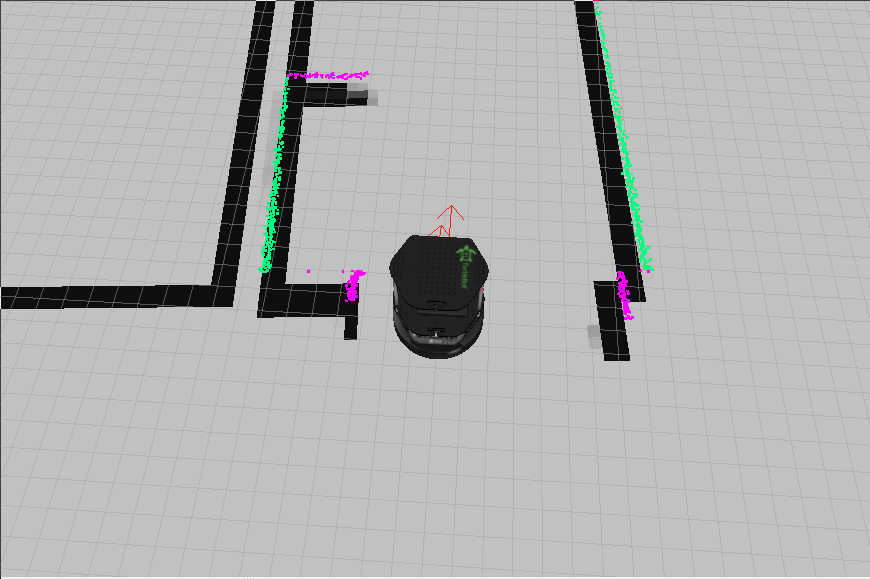
\includegraphics[width=10cm,height=7cm]{img/cap3/finamcl}
  \end{center}
  \caption{El robot se encuentra totalmente localizado}
  \label{fig:finamcl}
\end{figure}

En la imagen \ref{fig:finamcl} vemos como el número de partículas se ha reducido mucho, ya que se ha llegado a casi una estimación de la posición del robot muy cerca de la posición real. Vemos también que las lineas de color correspondientes a las muestras del láser están alineadas con el mapa.

Para el uso del paquete \textit{amcl} en nuestro algoritmo fue necesaria la realización de una pequeña modificación. Esta modificación se refiere a que el paquete por defecto solo usa un mapa y lo obtiene al principio de la ejecución del algoritmo. Si le llegaba un nuevo mapa reiniciaba por completo el algoritmo. Esto nos generaba un problema, ya que en el algoritmo propuesto se publica un mapa por cada iteración y el paquete por defecto se reiniciaba constantemente. El efecto que producía es que el robot siempre se encontraba en la posición inicial y aunque lo moviéramos siempre ocupaba la misma posición en el mapa. En nuestro \textit{amcl} modificado se usa el mapa que se obtiene en cada iteración y sobre el se calcula la posición del robot, sin reiniciar en ningún momento el algoritmo.

\subsection{Navigation}
\label{sec:navigation}
\textit{Navigation}\footnote{http://wiki.ros.org/navigation} es un conjunto de paquetes de ROS que toman información de la odometría, los sensores y la posición inicial y la posición a la que el robot tiene que llegar, ejecuta distintos algoritmos para calcular la ruta desde el punto inicial al final y ejecuta los comandos de movimiento necesarios para que el robot ejecute esa ruta.


\subsubsection{Move\_base}
\label{sec:movebase}
El paquete principal para la navegación es el paquete \textit{move\_base}\footnotemark. Este paquete es el encargado de, proporcionándole un punto de meta, calcular el plan necesario para llegar hasta dicho punto y ejecutar dicho plan para que el robot alcance su destino. \textit{Move\_base} cuenta con dos procesos o \textit{planners} que calculan y ejecutan la ruta, \textit{global} y \textit{local planner}. El global planner se encarga de planificar la ruta teniendo en cuenta el mapa que obtiene de nuestro algoritmo, por ejemplo, esquivará distintos objetos que haya en el mapa y planificará la ruta más rápida para llegar al destino. Además recalculará una nueva ruta si el robot se parara a causa de un objeto o si en medio del camino se da cuenta que la ruta no puede llevarse a cabo. 

El local planner se encarga de esquivar objetos que no están en el mapa y de navegar de una forma segura, sin chocar con las paredes o los muebles del escenario.
\footnotetext{http://wiki.ros.org/move\_base?distro=indigo}